\documentclass{beamer}
\usepackage[english,activeacute]{babel}
\usepackage[utf8]{inputenc}
\usepackage{listings}
\usepackage{color}
\usepackage{tikz}

\definecolor{red}{RGB}{255,0,0}
\definecolor{green}{RGB}{0,255,0} 
\definecolor{blue}{RGB}{0,0,255} 
\definecolor{oran}{RGB}{255,93,0} 

\newcommand{\blue}{\textcolor{blue}}
\newcommand{\red}{\textcolor{red}}
\newcommand{\green}{\textcolor{green}}
\newcommand{\oran}{\textcolor{oran}}

\usetheme[pageofpages=of,
          alternativetitlepage=true,
          titlepagelogo=img/cti_hpc-500,
          watermark=,
          watermarkheight=50px,
          watermarkheightmult=1,
          ]{Torino}

\usecolortheme{nouvelle}
\vspace{-0.5cm}
\author[Cristián D. Maureira Fredes]
       {\large Cristián D. Maureira Fredes\\
        \normalsize \textcolor{gray}{cmaureir@hpc.cl}}
\title[BH Integrator]
      {\Huge Black hole dynamics integrator}
\subtitle{
      A quasi-keplerian N-body
      gravitational system integration.
     }
\institute[UTFSM]
          {Universidad Técnica\\
           Federico Santa María}

\begin{document}
\begin{frame}[t,plain]
\titlepage
\end{frame}
\begin{frame}
    \frametitle{Introduction}
    \framesubtitle{Galactic center}
    \begin{figure}
        \centering
        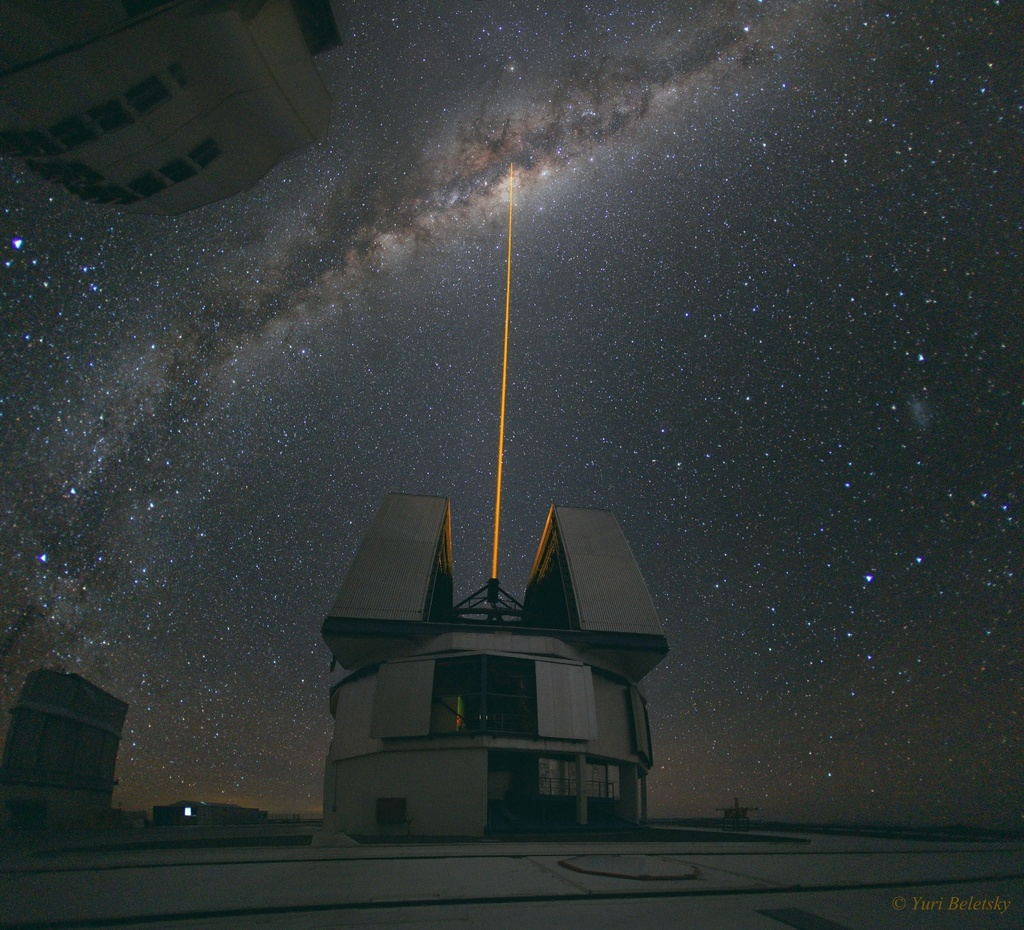
\includegraphics[width=0.55\textwidth]{img/galactic-center}
        \caption{A laser strike at the Galactic Center (Yuri Beletsky)}
        \label{fig:galactic-center}
    \end{figure}
\end{frame}

\begin{frame}
    \frametitle{Introduction}
    \framesubtitle{Galactic center}
    \begin{itemize}
        \item Rotational center of the Milky Way.
        \item Strong evidence about the existence of a SMBH.
            \item Astronomical radio source (Sagittarius A)
            \item BH diameter $\approx$ 0.3 AU
            \begin{itemize}
                \item $1 AU \approx 149\cdot10^{6} km$ 
            \end{itemize}
            \item BH mass $\approx 4\cdot 10^{6} M_{\odot}$
            \begin{itemize}
                \item $M_{\odot} \approx 1.9\cdot 10^{30} kg$
            \end{itemize}
    \end{itemize}
\end{frame}

\begin{frame}
    \frametitle{Introduction}
    \framesubtitle{The puzzle}
    \begin{itemize}
        \item Population of young massive stars (~5 Myr) orbiting a fraction of a pc.
        \begin{itemize}
            \item $1 pc \approx 3.1\cdot 10^{13} km$
        \end{itemize}
        \item Their existence is a puzzle.
        \begin{itemize}
            \item Tidal field prevents star formation.
            \item Isotropic orbits (S-stars).
            \item Many stars lie on a single plane.
        \end{itemize}
        \item Big question: \blue{"How this disc was formed?"}
    \end{itemize}
\end{frame}

\begin{frame}
    \frametitle{Introduction}
    \framesubtitle{Formation theories}
    Two main theories:
    \begin{enumerate}
        \item Inside the accretion disc, exceeding the tidal limit.
        \item Outside the GC but migrated to the disc.
    \end{enumerate}
\end{frame}

\begin{frame}
    \frametitle{Problem}
    \framesubtitle{Approach}

    \begin{itemize}
        \item Considering the first theory.
        \begin{itemize}
            \item Study the dynamical evolution from any plausible
                  cold disc initial conditions.
            \begin{itemize}
                \item Single stars.
                \item Primordial binaries.
                \item Eccentric flat disc.
                \item Massive stars.
                \item Intermediate mass BH.
            \end{itemize}
        \end{itemize}
    \end{itemize}

    \emph{``Stellar dynamical evidence against a cold disc origin
    for stars in the Galactic Centre''} (Cuadra et al).
\end{frame}

\begin{frame}
    \frametitle{Problem}
    \framesubtitle{Approach}
    \begin{itemize}
        \item The previous work was developed using:
        \begin{itemize}
            \item CPU simulation environment.
            \item $100$ disc stars.
            \item Bulirsch-Stoer integrator (conservative systems).
            \item $2700$ orbits.
            \item $r = 0.1 pc$.
        \end{itemize}
    \end{itemize}
\end{frame}

\begin{frame}
    \frametitle{Problem}
    \framesubtitle{Discussion}
    \begin{itemize}
        \item Unrealistic environment.
        \begin{itemize}
            \item Ignoring low mass stars.
            \item Including only the observed population of stars in the GC.
        \end{itemize}
        \item CPU restrictions.
    \end{itemize}
\end{frame}

\begin{frame}
    \frametitle{Proposal}
    \framesubtitle{Issues to consider}

    \begin{itemize}
        \item Stellar systems around SMBHs $\approx$ Planetary system.
        \begin{itemize}
            \item Stars with ``weakly'' perturbed keplerian orbits.
        \end{itemize}
        \item But also, a SMBH system is like a star cluster.
        \begin{itemize}
            \item Different eccentricities ranges.
            \item Similar mass stars.
        \end{itemize}
    \end{itemize}
\end{frame}


\begin{frame}
    \frametitle{Proposal}
    \framesubtitle{Existing solution (CPU)}
    \begin{itemize}
        \item \texttt{bhint} by Ulf Löckmann (Universität Bonn)
        \item Combination of:
        \begin{itemize}
            \item High precision of Keplerian orbital motion
            \item High speed and flexibility of N-body integrator
        \end{itemize}
        \item Features
        \begin{itemize}
            \item Post-Newtonian extension (relativistic effects).
            \item Close encounters special treatment.
        \end{itemize}
    \end{itemize}
\end{frame}

\begin{frame}
    \frametitle{Future Work}
    \framesubtitle{a lot!}
    \begin{itemize}
        \item Understand:
        \begin{itemize}
            \item Symplectic and Non-symplectic integration schemes.
            \begin{itemize}
                \item Kepler's equation.
                \item Hermite scheme.
                \item Hamiltonian systems.
                \item Bulirsch-Stoer algorithm.
                \item Relativistic effects.
                \item etc.
            \end{itemize}
        \end{itemize}
    \end{itemize}
\end{frame}

\begin{frame}[t,plain]
\titlepage
\end{frame}
\end{document}
